\documentclass[tikz,border=5pt]{standalone}
\pdfinfoomitdate=1
\pdftrailerid{}
\pdfsuppressptexinfo=-1
\usepackage{pgfplots}
\usepgfplotslibrary{groupplots}
\pgfplotsset{compat=1.18}
\definecolor{atlasBlue}{HTML}{0072B2}
\definecolor{atlasOrange}{HTML}{E69F00}
\definecolor{atlasGreen}{HTML}{009E73}
\definecolor{atlasPurple}{HTML}{CC79A7}
\definecolor{atlasGray}{HTML}{777777}
% NATO SERS figure F45; data_sha256=ca4e573fb6075e3e884e90a68e5b594d815d3bb6ba9873db7ac825428a51ae79
% title=Held-instrument analyte recoverability by substrate
% caption=C-SELECTED with PP-U-MIN. Points and horizontal bars are estimates and 95\% master-clustered bootstrap intervals. Portability requires held balanced-accuracy LCB at least 0.60 and matched source-minus-held loss UCB at most 0.10. Open gray marks at the plot boundary are predeclared unavailable endpoints. n is physical masters.
\begin{document}
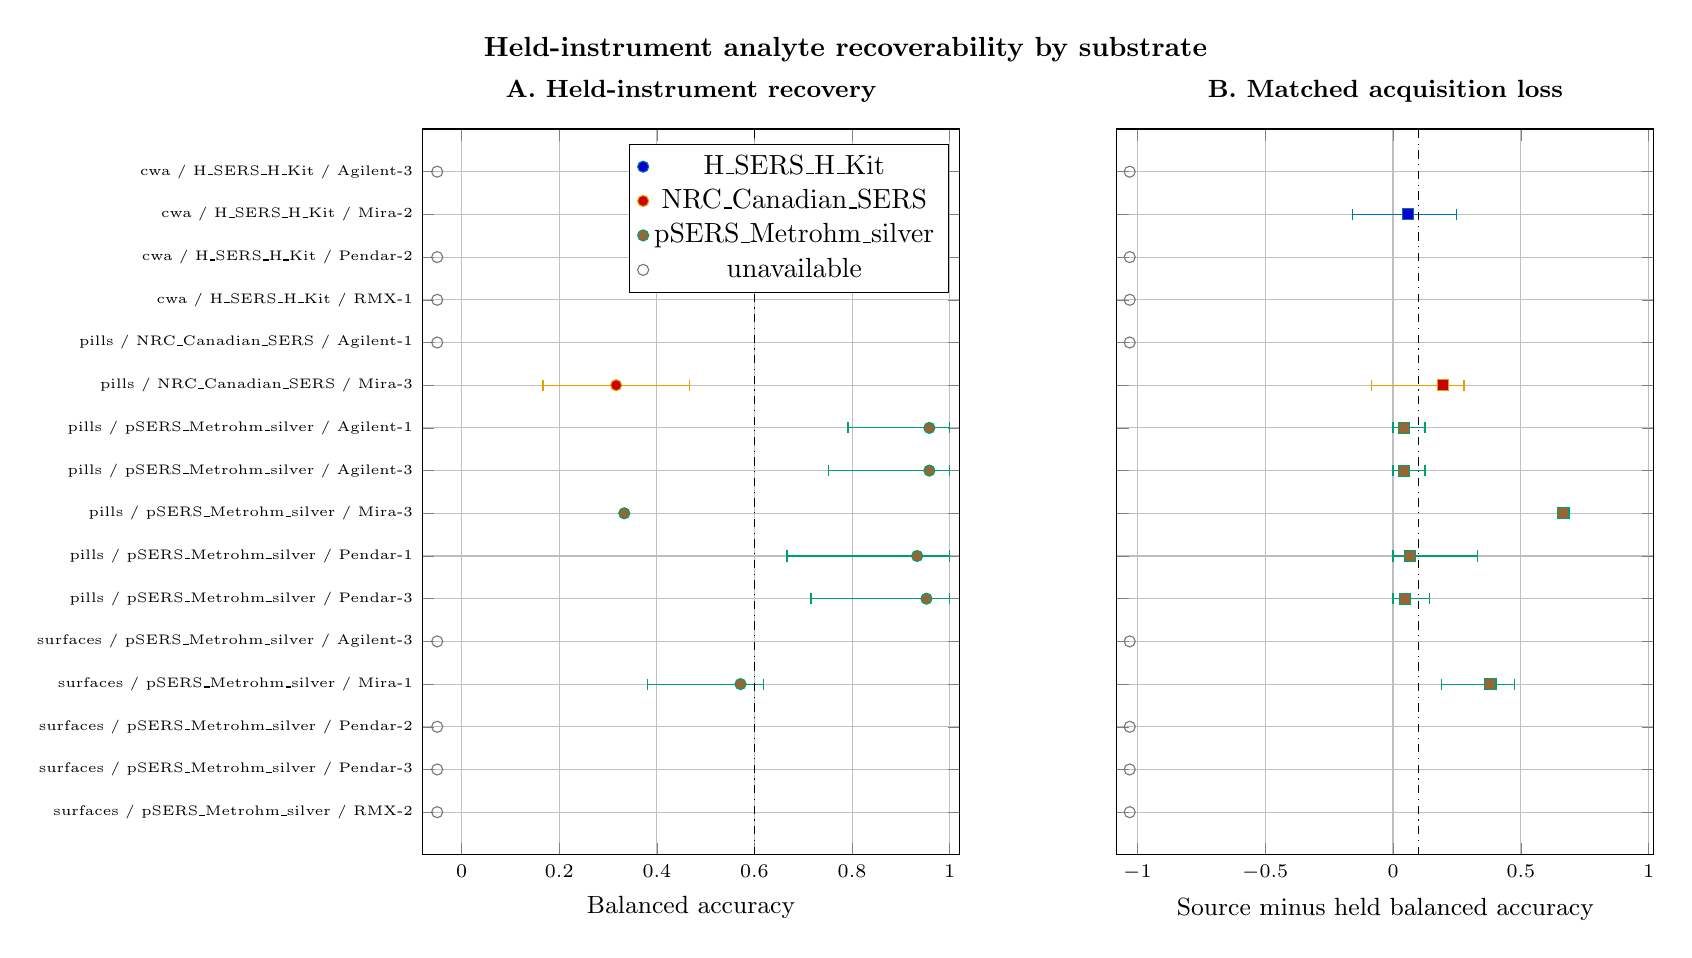
\begin{tikzpicture}
\begin{groupplot}[group style={group size=2 by 1,horizontal sep=2.0cm},width=8.4cm,height=10.8cm,
tick label style={font=\scriptsize},label style={font=\small},title style={font=\small\bfseries},
ytick={15,14,13,12,11,10,9,8,7,6,5,4,3,2,1,0},yticklabels={cwa / H\_SERS\_H\_Kit / Agilent-3,cwa / H\_SERS\_H\_Kit / Mira-2,cwa / H\_SERS\_H\_Kit / Pendar-2,cwa / H\_SERS\_H\_Kit / RMX-1,pills / NRC\_Canadian\_SERS / Agilent-1,pills / NRC\_Canadian\_SERS / Mira-3,pills / pSERS\_Metrohm\_silver / Agilent-1,pills / pSERS\_Metrohm\_silver / Agilent-3,pills / pSERS\_Metrohm\_silver / Mira-3,pills / pSERS\_Metrohm\_silver / Pendar-1,pills / pSERS\_Metrohm\_silver / Pendar-3,surfaces / pSERS\_Metrohm\_silver / Agilent-3,surfaces / pSERS\_Metrohm\_silver / Mira-1,surfaces / pSERS\_Metrohm\_silver / Pendar-2,surfaces / pSERS\_Metrohm\_silver / Pendar-3,surfaces / pSERS\_Metrohm\_silver / RMX-2},y tick label style={font=\tiny,align=right},grid=major]
\nextgroupplot[title={A. Held-instrument recovery},xlabel={Balanced accuracy},xmin=-0.08,xmax=1.02,ymin=-1,ymax=16,xmajorgrids=true]
\addplot+[only marks,mark=*,color=atlasBlue,error bars/.cd,x dir=both,x explicit] coordinates {(0.70899471,14) += (0.14285714,0) -= (0.17989418,0)};
\addlegendentry{H\_SERS\_H\_Kit}
\addplot+[only marks,mark=*,color=atlasOrange,error bars/.cd,x dir=both,x explicit] coordinates {(0.31666667,10) += (0.15,0) -= (0.15,0)};
\addlegendentry{NRC\_Canadian\_SERS}
\addplot+[only marks,mark=*,color=atlasGreen,error bars/.cd,x dir=both,x explicit] coordinates {(0.95833333,9) += (0.041666667,0) -= (0.16666667,0) (0.95833333,8) += (0.041666667,0) -= (0.20727166,0) (0.33333333,7) += (0,0) -= (0,0) (0.93333333,6) += (0.066666667,0) -= (0.26666667,0) (0.95238095,5) += (0.047619048,0) -= (0.2365925,0) (0.57142857,3) += (0.047619048,0) -= (0.19047619,0)};
\addlegendentry{pSERS\_Metrohm\_silver}
\addplot+[only marks,mark=o,color=atlasGray] coordinates {(-0.05,15) (-0.05,13) (-0.05,12) (-0.05,11) (-0.05,4) (-0.05,2) (-0.05,1) (-0.05,0)};\addlegendentry{unavailable}
\addplot[black,dashdotted] coordinates {(0.6,-1) (0.6,16)};
\nextgroupplot[title={B. Matched acquisition loss},xlabel={Source minus held balanced accuracy},xmin=-1.08,xmax=1.02,ymin=-1,ymax=16,yticklabels={},xmajorgrids=true]
\addplot+[only marks,mark=square*,color=atlasBlue,error bars/.cd,x dir=both,x explicit] coordinates {(0.058862434,14) += (0.18981481,0) -= (0.21693122,0)};
\addplot+[only marks,mark=square*,color=atlasOrange,error bars/.cd,x dir=both,x explicit] coordinates {(0.19444444,10) += (0.083333333,0) -= (0.27777778,0)};
\addplot+[only marks,mark=square*,color=atlasGreen,error bars/.cd,x dir=both,x explicit] coordinates {(0.041666667,9) += (0.083333333,0) -= (0.041666667,0) (0.041666667,8) += (0.083333333,0) -= (0.041666667,0) (0.66666667,7) += (0,0) -= (0,0) (0.066666667,6) += (0.26216193,0) -= (0.066666667,0) (0.047619048,5) += (0.095238095,0) -= (0.047619048,0) (0.38095238,3) += (0.095238095,0) -= (0.19047619,0)};
\addplot+[only marks,mark=o,color=atlasGray] coordinates {(-1.03,15) (-1.03,13) (-1.03,12) (-1.03,11) (-1.03,4) (-1.03,2) (-1.03,1) (-1.03,0)};
\addplot[black,dashdotted] coordinates {(0.1,-1) (0.1,16)};
\end{groupplot}
\node[font=\normalsize\bfseries,anchor=south] at (current bounding box.north) {Held-instrument analyte recoverability by substrate};
\end{tikzpicture}
\end{document}
